\documentclass[a4paper,14pt]{article}
\usepackage[utf8]{inputenc}
\usepackage[english,russian]{babel}
\usepackage[T1, T2A]{fontenc}
\usepackage{graphicx}
\usepackage{epstopdf}
\usepackage{caption}
\usepackage[margin=14pt,font=small,labelsep=endash]{caption}

\usepackage{float}
\usepackage{geometry} %способ ручной установки полей
\geometry{top=2cm} %поле сверху
\geometry{bottom=2cm} %поле снизу
\geometry{left=2cm} %поле справа
\geometry{right=2cm} %поле слева


%opening
%\title{}
%\author{}

\begin{document}
%\maketitle
\textbf {Цель работы:} исследование точностных свойств систем управления.
\section{Исследование системы с астатизмом нулевого порядка.}
Таблица 1 - Вариант параметров системы с нулевым порядком астатизма. 

\begin{center}
\begin{tabular}{ |c|c|c|c| } 
 \hline
 Вариант & W(s) & g(t)=A & g(t)=Vt \\ 
 \hline
 9 & $ 2/(0.5s^2+s+2) $ & 2 & 2t \\ 
 \hline
\end{tabular}
\end{center}

\paragraph{Иследование стационарного режима работы: g(t)=A.}
Значение коэффициентов k: 1, 5, 10.
На рисунке 1 представлена структурная схема моделируемой системы.
\begin{figure}[h!]
\centering
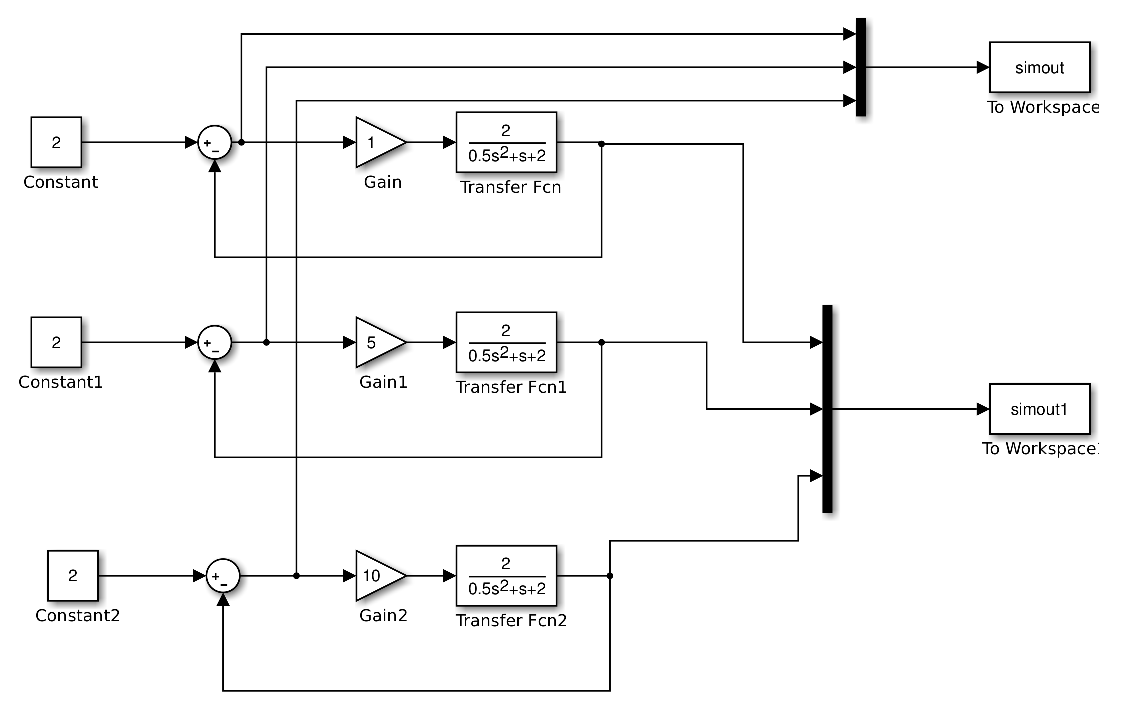
\includegraphics[width=\textwidth]{1/1_1.eps}
\caption{Структурная схема моделируемой  системы.}
\end{figure}

Получили переходные процессы для трех различных значений коэффициентов k (k=1; k=5; k=10).
На рисунке 2 представлены графики переходного процесса для k=1; k=5; k=10.
\begin{figure}[H]
\centering
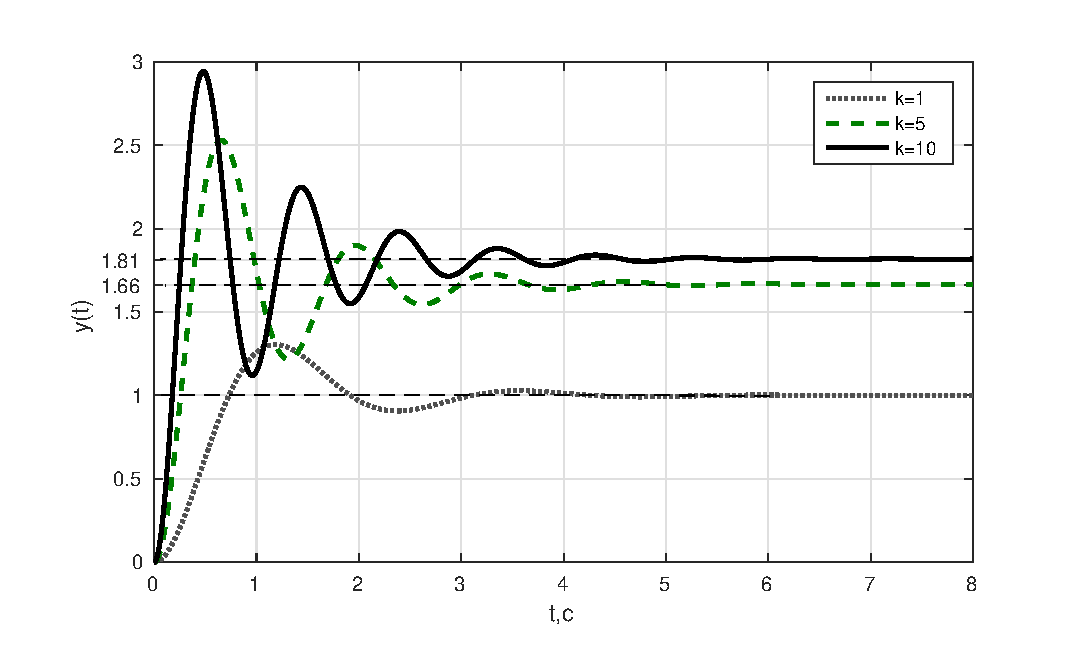
\includegraphics[width=\textwidth]{1/1_1y(t).eps}
\caption{Графики переходного процесса для k=1; k=5; k=10.}
\end{figure}

Было получено предельное значение установившейся ошибки е. На рисунке 3 приведены графики, изображающие предельное значение установившейся ошибки. 
\begin{figure}[H]
\centering
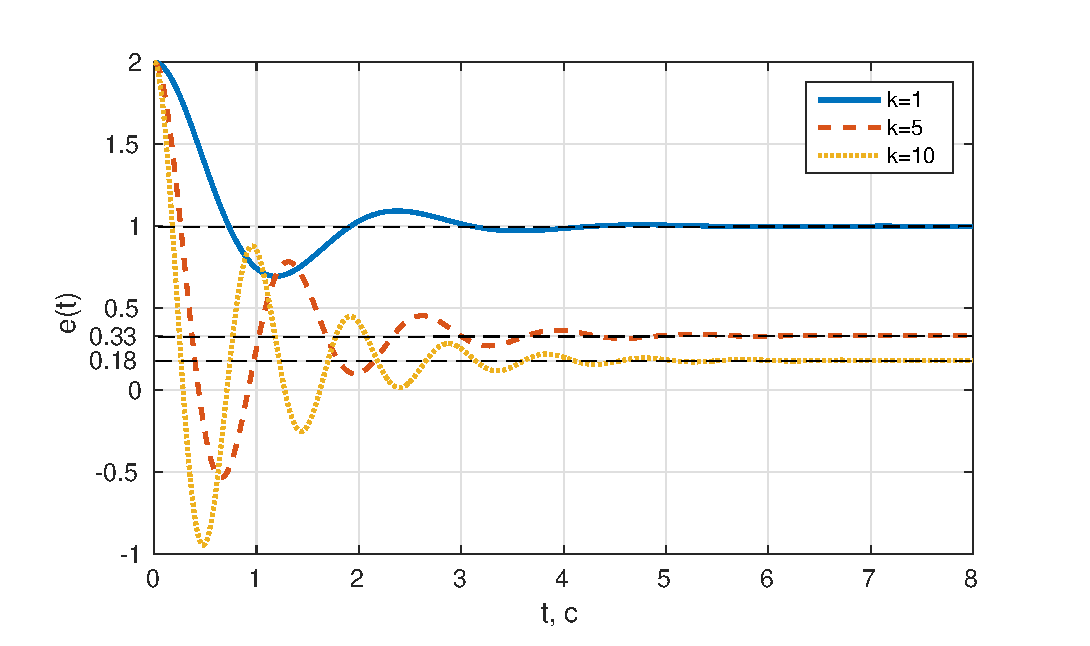
\includegraphics[width=\textwidth]{1/1_1e.eps}
\caption{Графики, изображающие предельное значение установившейся ошибки.}
\end{figure}

С помощью расчета проверим получившееся на графике значения установившейся ошибки:
\begin{equation}
e=A/(1+k)
\end{equation}
\\при k=1: e=A/(1+k)=2/(1+1)=1
\\при k=5: e=2/6=1/3=0,33
\\при k=10: e=2/11=0,18.
\\Рассчитанные значения совпадают с получившимися значениями на графике.

\paragraph{Исследование режима движения с постоянной скоростью: g(t)=Vt.}
На рисунке 4 представлена структурная схема моделируемой системы.
\begin{figure}[H]
\centering
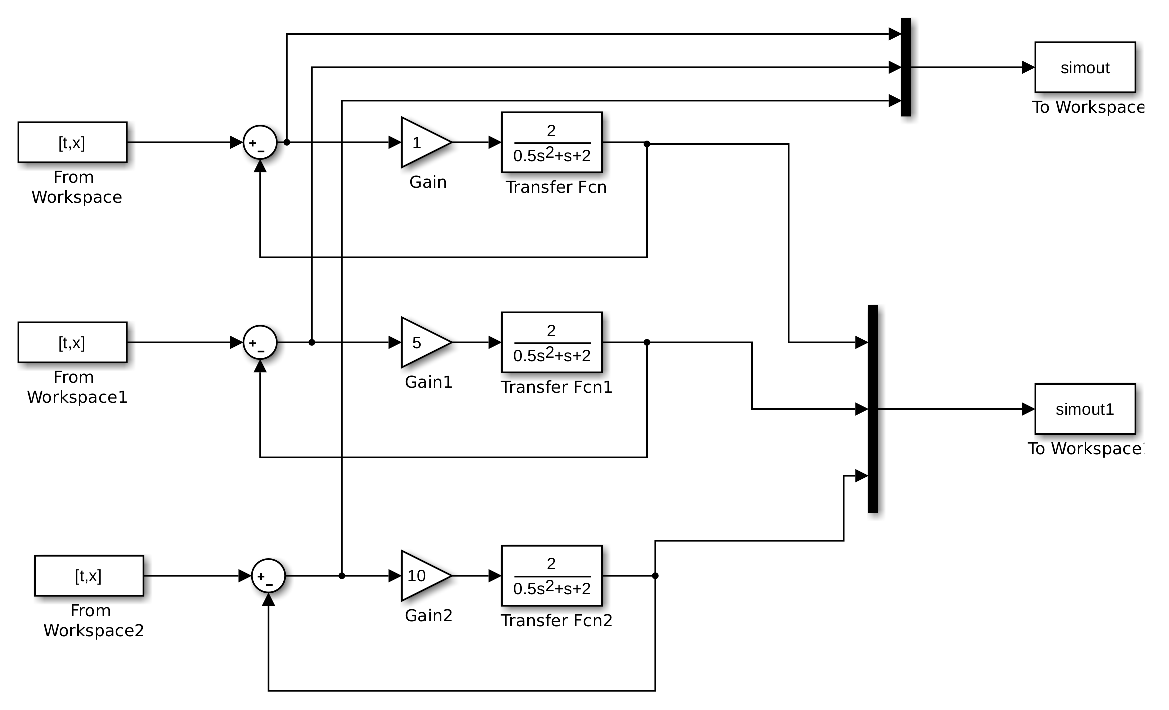
\includegraphics[width=\textwidth]{1/1_2.eps}
\caption{Структурная схема моделируемой  системы.}
\end{figure}

Получили переходные процессы для трех различных значений коэффициентов k (k=1; k=5; k=10).
\begin{figure}[H]
\centering
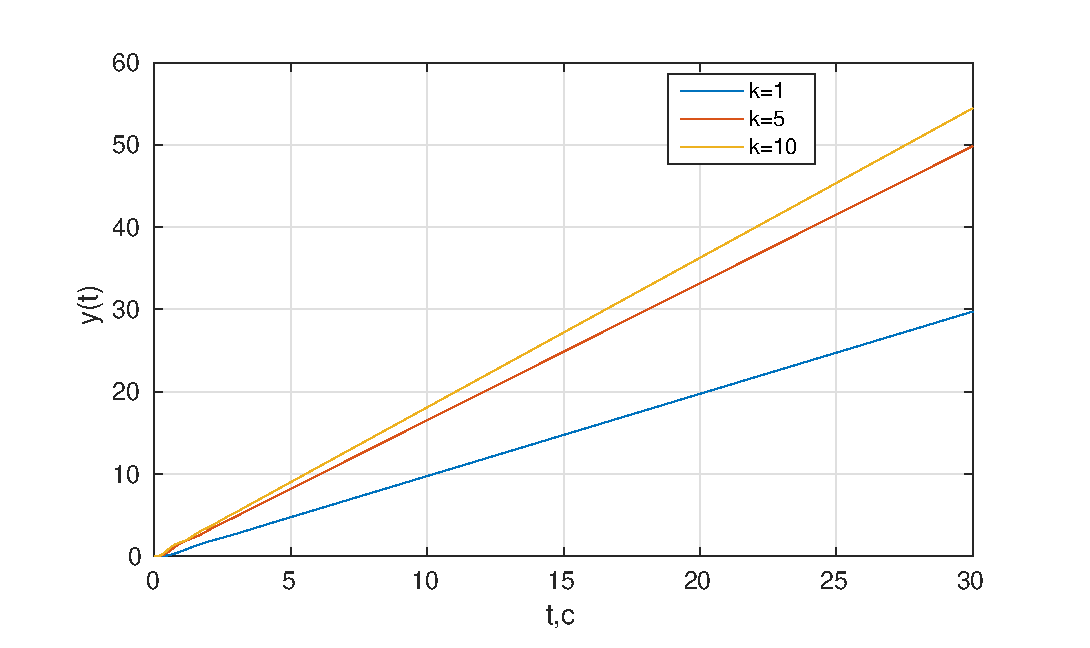
\includegraphics[width=\textwidth]{1/1_2y(t).eps}
\caption{Графики переходного процесса для k=1; k=5; k=10.}
\end{figure}

\newpage
\section {Исследование системы с астатизмом первого порядка.}
Таблица 2 - Вариант параметров системы с первым порядком астатизма. 
\begin{center}
\begin{tabular}{ |c|c|c| } 
 \hline
 Вариант & W(s) & $g=at^2/2$  \\ 
 \hline
 9 & $ (s+2)/(0.5s^2+s+2) $ & $0.5t^2$  \\ 
 \hline
\end{tabular}
\end{center}

\paragraph{Исследование стационарного режима работы: g(t)= A.}
На рисунке 6 представлена структурная схема моделируемой системы.

\begin{figure}[H]
\centering
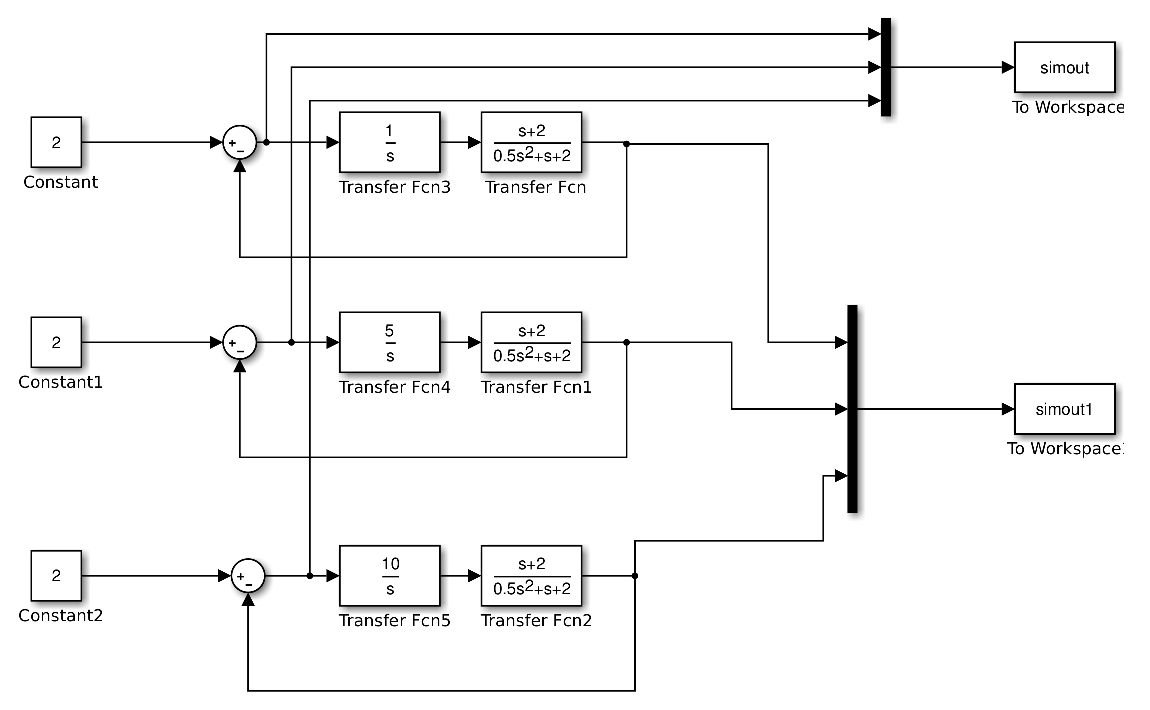
\includegraphics[width=\textwidth]{1/cxema_2.eps}
\caption{Структурная схема моделируемой  системы.}
\end{figure}
Были получены переходные процессы для различных значений коэффициента  k.
На рисунке 6 приведены графики переходных процессов  для различных значений коэффициента  k.

\begin{figure}[H]
\centering
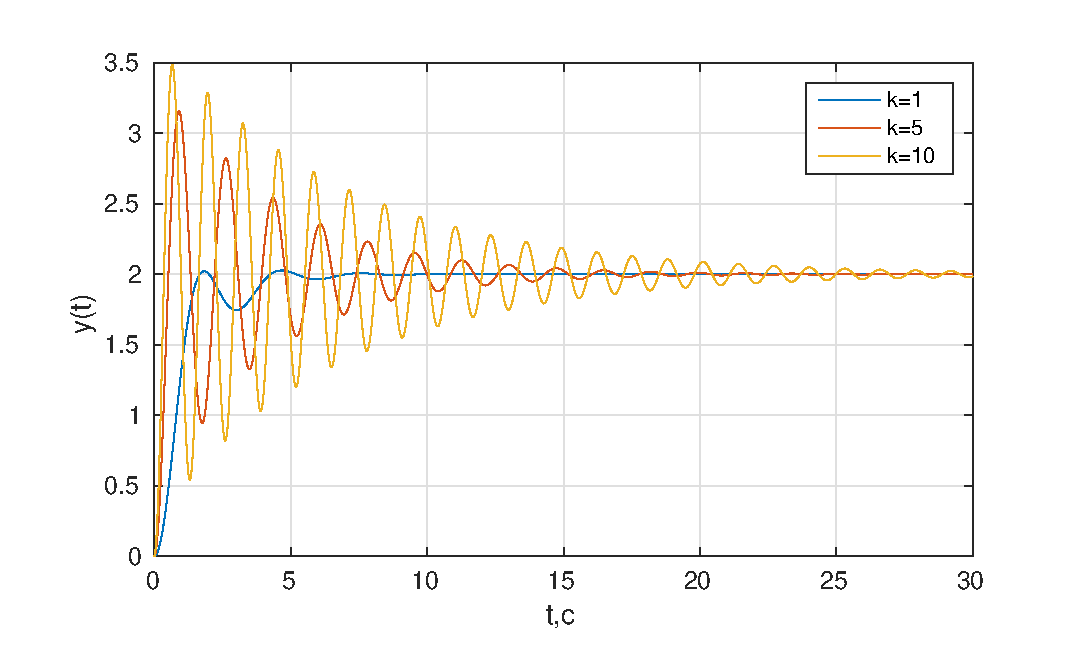
\includegraphics[width=\textwidth]{1/2_1y(t).eps}
\caption{Графики переходного процесса для k=1; k=5; k=10.}
\end{figure}
Было получено предельное значение установившейся ошибки е.

\begin{figure}[H]
\centering
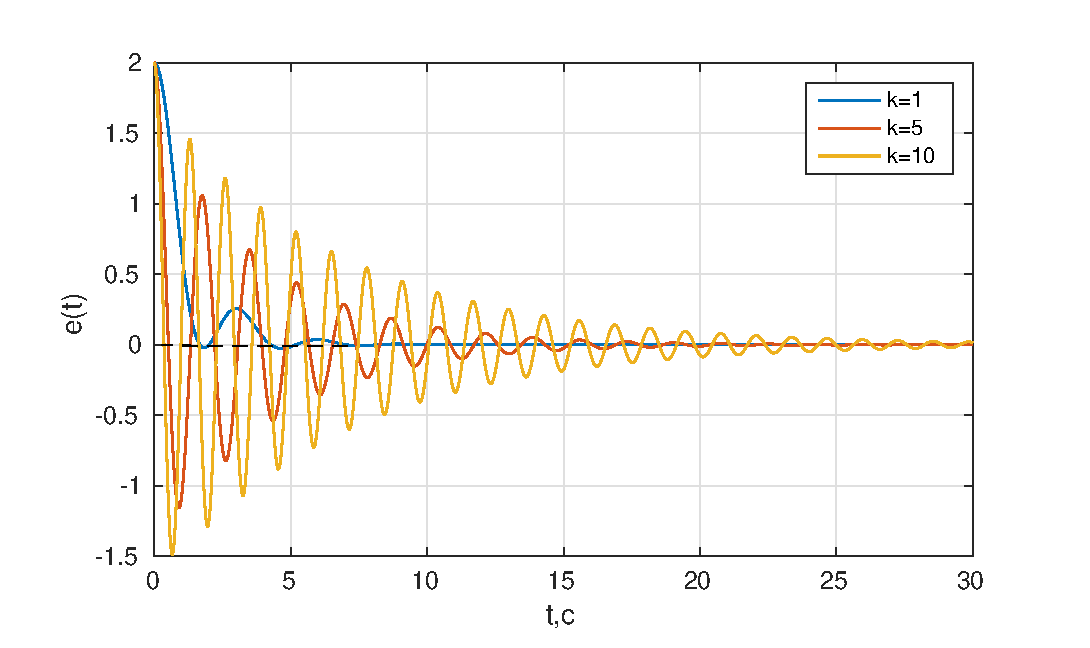
\includegraphics[width=\textwidth]{1/2_1e(t).eps}
\caption{Графики, изображающие предельное значение установившейся ошибки.}
\end{figure}

Для системы с астатизмом 1 порядка значение установившейся ошибки е=0 (при g(t)=A).

\paragraph{Исследование режима движения с постоянной скоростью: $g(t)=Vt$.}
Были получены переходные процессы для различных значений коэффициента  k.
На рисунке 8 приведены графики переходных процессов  для различных значений коэффициента  k.

\begin{figure}[H]
\centering
\includegraphics[width=\textwidth]{1/2_2y(t).eps}
\caption{Графики переходного процесса для k=1; k=5; k=10.}
\end{figure}
Было получено предельное значение установившейся ошибки е.

\begin{figure}[H]
\centering
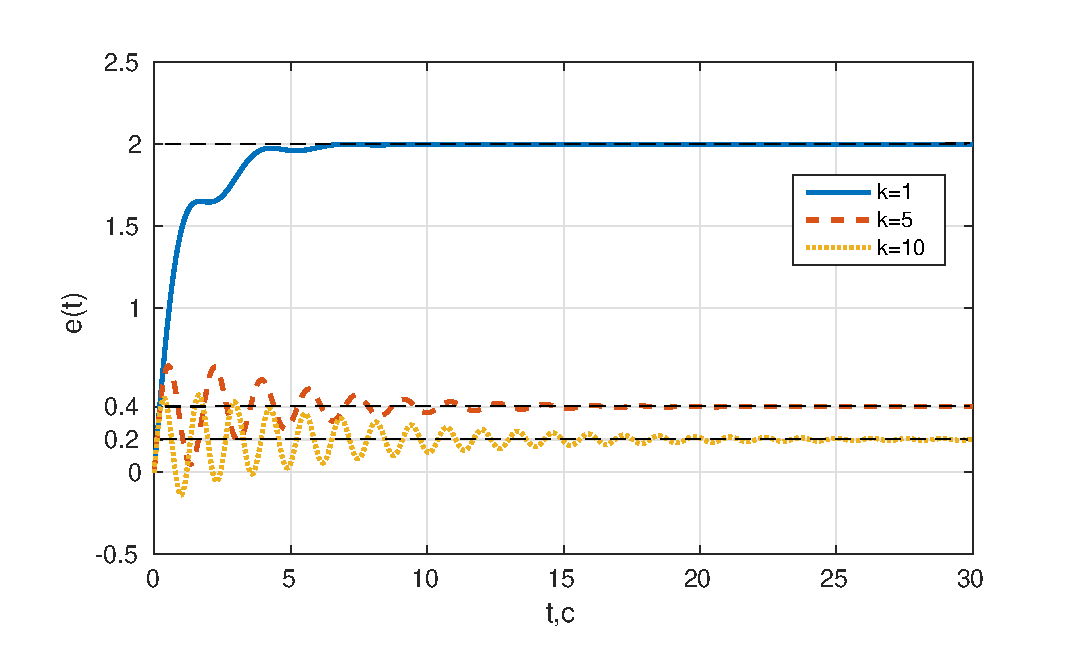
\includegraphics[width=\textwidth]{1/2_2e(t).eps}
\caption{Графики, изображающие предельное значение установившейся ошибки.}
\end{figure}

Из рисунка видно, что 
\\при k=1:  e=2
\\при k=5: е=0,4
\\при k=10: е=0,2.

С помощью расчета проверим получившееся на графике значения установившейся ошибки:
\begin{equation}
e=V/k
\end{equation}
\\при k=1: e=V/k=2/1=2
\\при k=5: e=2/5=0,4
\\при k=10: e=2/10=0,2
\\Рассчитанные значения совпадают с получившимися значениями на графике.

\paragraph{Исследование режима движения с постоянным ускорением: $g(t)=at^2/2$.}
Были получены переходные процессы для различных значений коэффициента  k.
\\На рисунке 10 приведены графики переходных процессов  для различных значений коэффициента  k.

\begin{figure}[H]
\centering
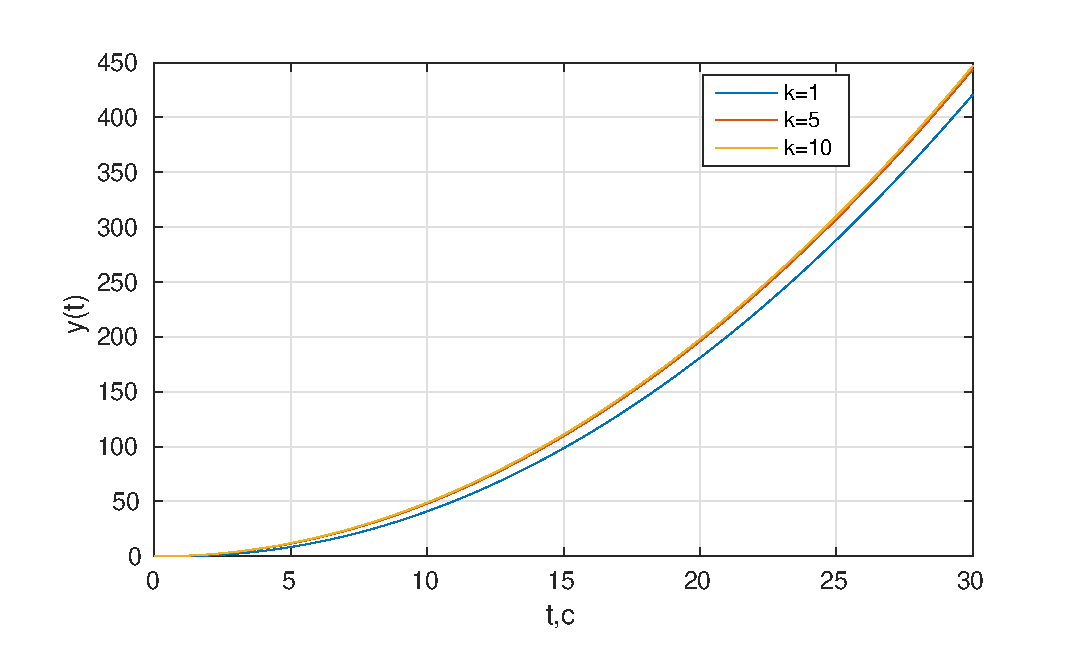
\includegraphics[width=\textwidth]{1/2_3y(t).eps}
\caption{Графики переходного процесса для k=1; k=5; k=10.}
\end{figure}

\newpage
\section{Исследование влияния внешних возмущений.}
Таблица 3 - Вариант возмущенной системы.

\begin{center}
\begin{tabular}{ |c|c| } 
 \hline
 $f_{1}$ & 2 \\ 
 \hline
 $f_{2}$ & 0.5 \\ 
 \hline
\end{tabular}
\end{center}
На рисунке 11 приведена схема моделирования возмущенной системы.

\begin{figure}[H]
\centering
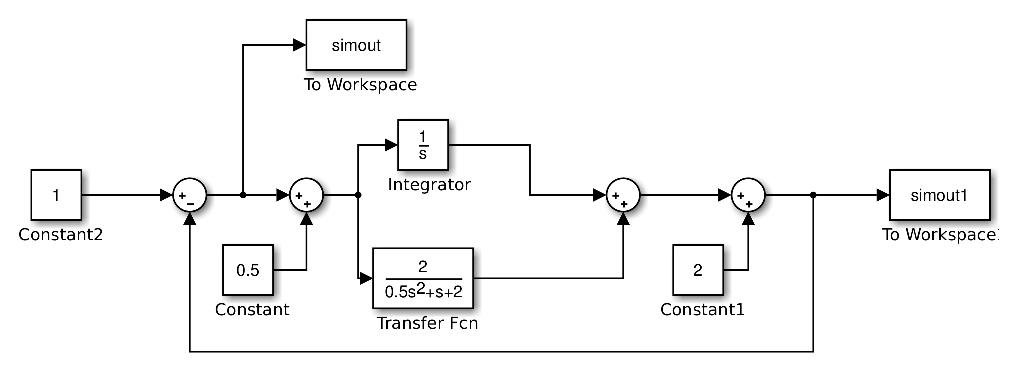
\includegraphics[width=\textwidth]{1/3.eps}
\caption{Схема моделирования возмущенной системы.}
\end{figure}


Положим $f_{2}(t)=0$ и g(t)=1(t), получим переходной процесс:

\begin{figure}[H]
\centering
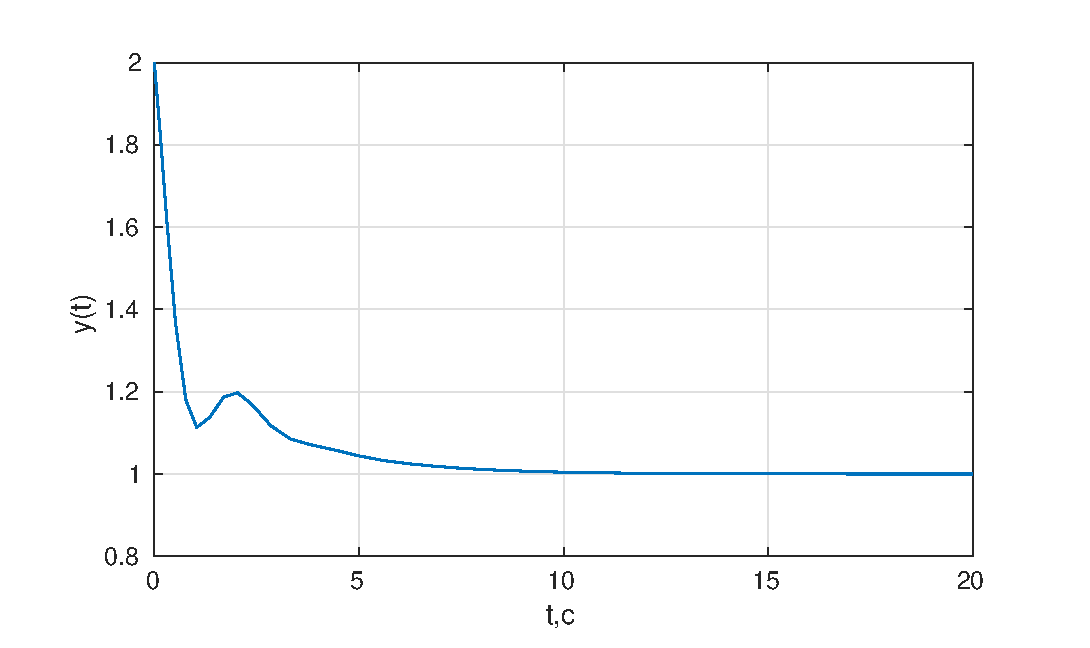
\includegraphics[width=\textwidth]{1/3_2y(t).eps}
\caption{График переходного процесса.}
\end{figure}

Было получено предельное значение установившейся ошибки е.

\begin{figure}[H]
\centering
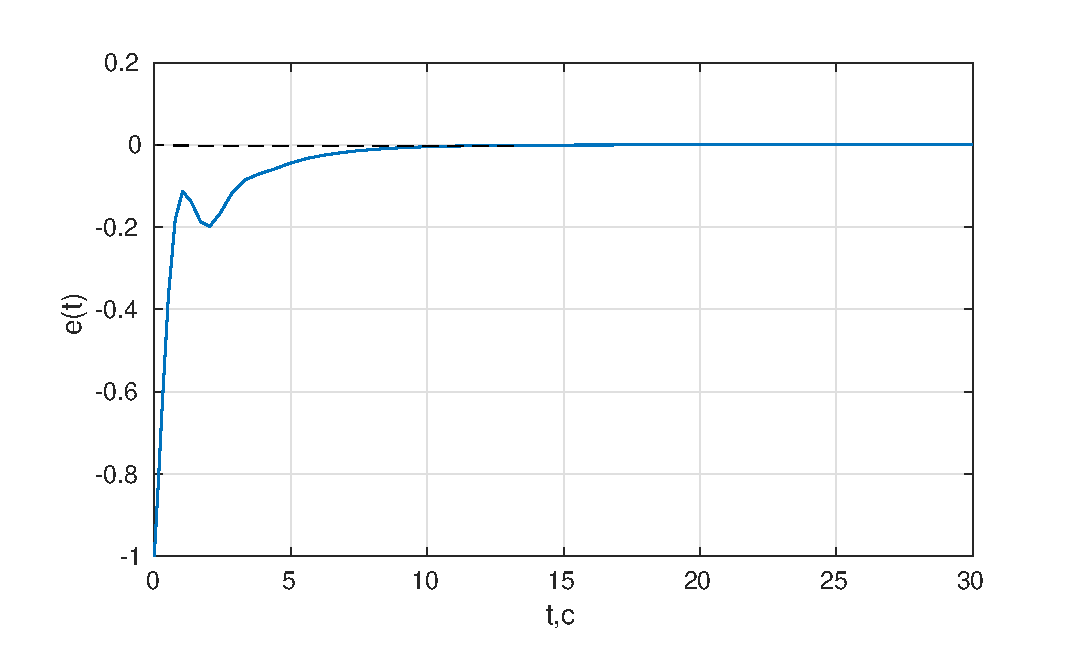
\includegraphics[width=\textwidth]{1/3_2e(t).eps}
\caption{График, изображающий предельное значение установившейся ошибки.}
\end{figure}
Предельное значение установившейся ошибки е=0.

Положим $f_{1}(t)=0$ и g(t)=1(t), получим переходной процесс:

\begin{figure}[H]
\centering
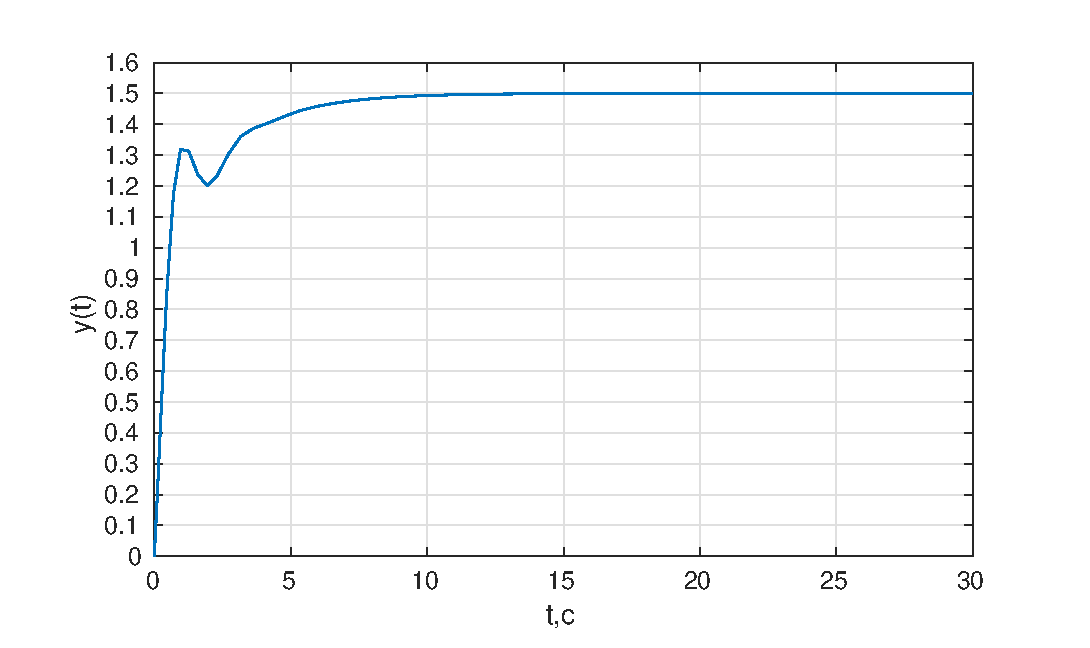
\includegraphics[width=\textwidth]{1/3_3y(t).eps}
\caption{График переходного процесса.}
\end{figure}

Было получено предельное значение установившейся ошибки е.
\begin{figure}[H]
\centering
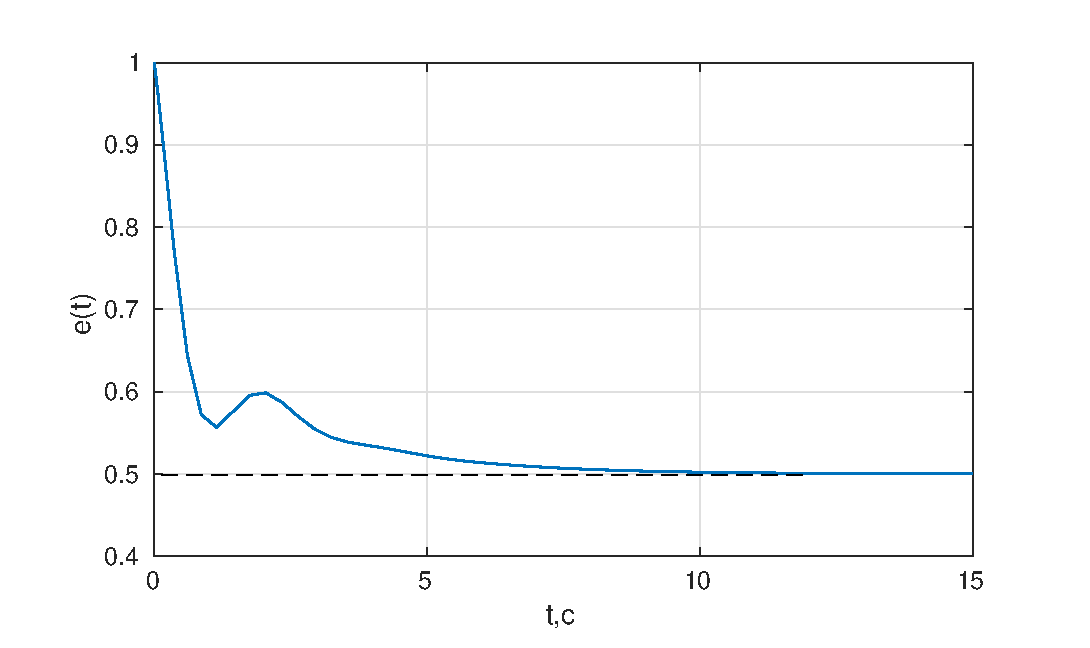
\includegraphics[width=\textwidth]{1/3_3e(t).eps}
\caption{График, изображающий предельное значение установившейся ошибки.}
\end{figure}

Предельное значение установившейся ошибки е=0,5.
\\Проверим полученное значение:
\begin{equation}
e=F_{2}=f_{2}(t)
\end{equation}
\\е=$F_{2}$=$f_{2}(t)$=0,5
\\Полученные значения установившейся ошибки сходятся, из этого можно сделать вывод, что полученное значение на графике — верно.

\newpage
\section{Исследование установившейся ошибки при произвольном входном воздействии.}

Таблица 3 - Вариант возмущенной системы.

\begin{center}
\begin{tabular}{ |c|c| } 
 \hline
Вариант & Сигнал задания \\ 
 \hline
 9 & $ 2+0.1t^2 $ \\ 
 \hline
\end{tabular}
\end{center}

Была собрана структурная схема данной системы:

\begin{figure}[H]
\centering
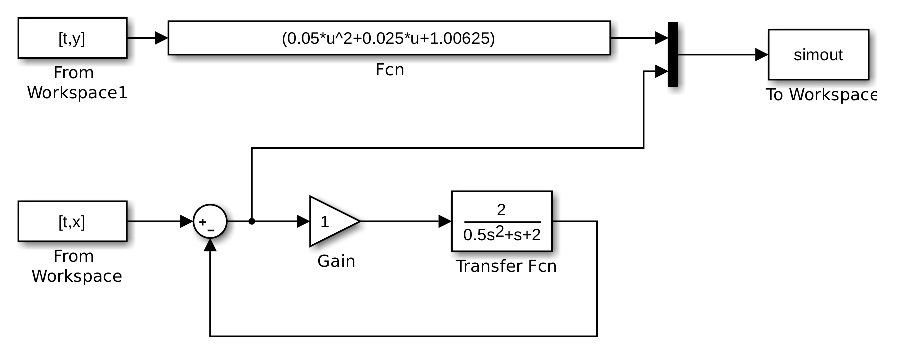
\includegraphics[width=\textwidth]{1/4.eps}
\caption{Структурная схема моделируемой  системы.}
\end{figure}
Был получен переходный процесс в замкнутой системе:


\begin{figure}[H]
\centering
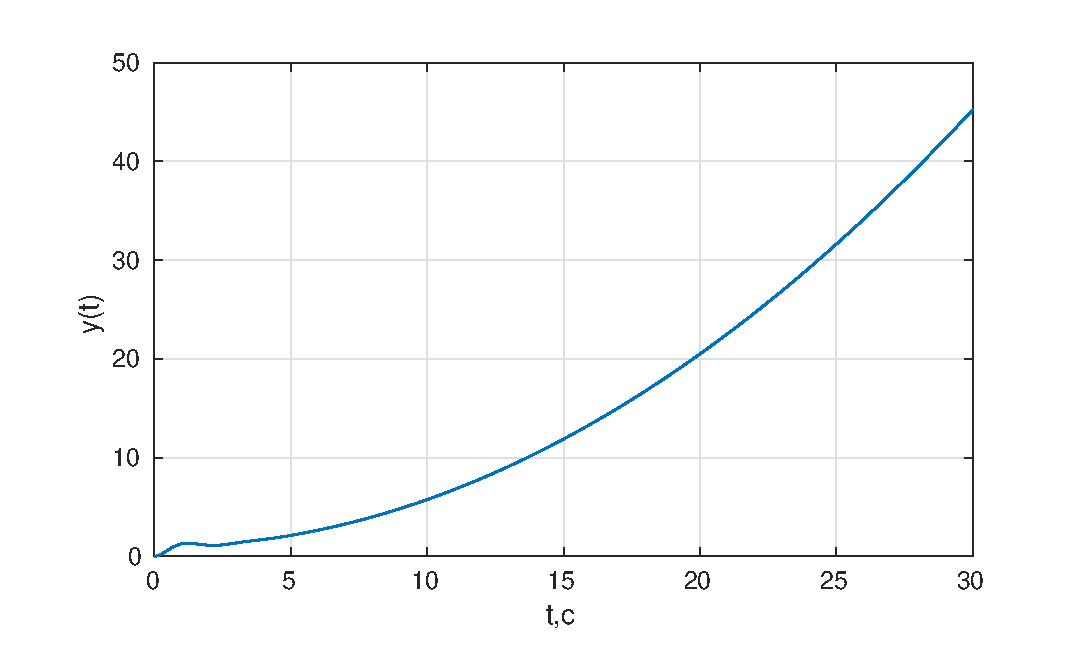
\includegraphics[width=\textwidth]{1/4_1y(t).eps}
\caption{Переходной процесс в замкнутой системе.}
\end{figure}

На рисунке 19 представлен график, изображающий  установившуюся ошибку слежения.
\begin{figure}[H]
\centering
\includegraphics[width=\textwidth]{1/4_1e(t).eps}
\caption{График, изображающий  установившуюся ошибку слежения.}
\end{figure}

Из графика видно, что установившаяся ошибка е=${\infty}$.

Получим приближенное аналитическое выражение для $e_{y}(t)$ , сохранив в ряде Тейлора три первых члена:
\begin{equation}
e(t)=c_{0}*g(t)+c_{1}*\dot{g}(t)+c_{2}/2!*\ddot{g}(t)
\end{equation}
\begin{equation}
c_{i}=[\frac{d^i}{ds^i}\Phi_{e}(s)]
\end{equation}
\\
\\$c_{0}=\Phi_{e}(s)=\frac{0.5s^2+s+2}{0.5s^2+s+4}$			
\\$g(t)=2+0.1t^2$
\\
\\при $s=0: c_{0}=0.5$
\\
\\$c_{1}=\dot\Phi_{e}(s)=\frac{d}{ds}\frac{0.5s^2+s+2}{0.5s^2+s+4}=\frac{8s+8}{(s^2+2s+8)^2}$		
\\$\dot{g}(t)=0.2t$
\\
\\при $s=0: c_{1}=0.125$
\\
\\$c_{2}=\ddot\Phi_{e}(s)=\frac{-24s^2-48s+32}{(s^2+2s+8)^3}$		
\\$\ddot{g}(t)=0.2$
\\
\\при $s=0: c_{2}=0.0625$
\\
\\ Подставим получившееся значения в выражение для ошибки:
\\$e(t)=0.05t^2+0.025t+1.00625$
\\ Получили графики  расчетной ошибки  и экспериментальной ошибки.

\begin{figure}[H]
\centering
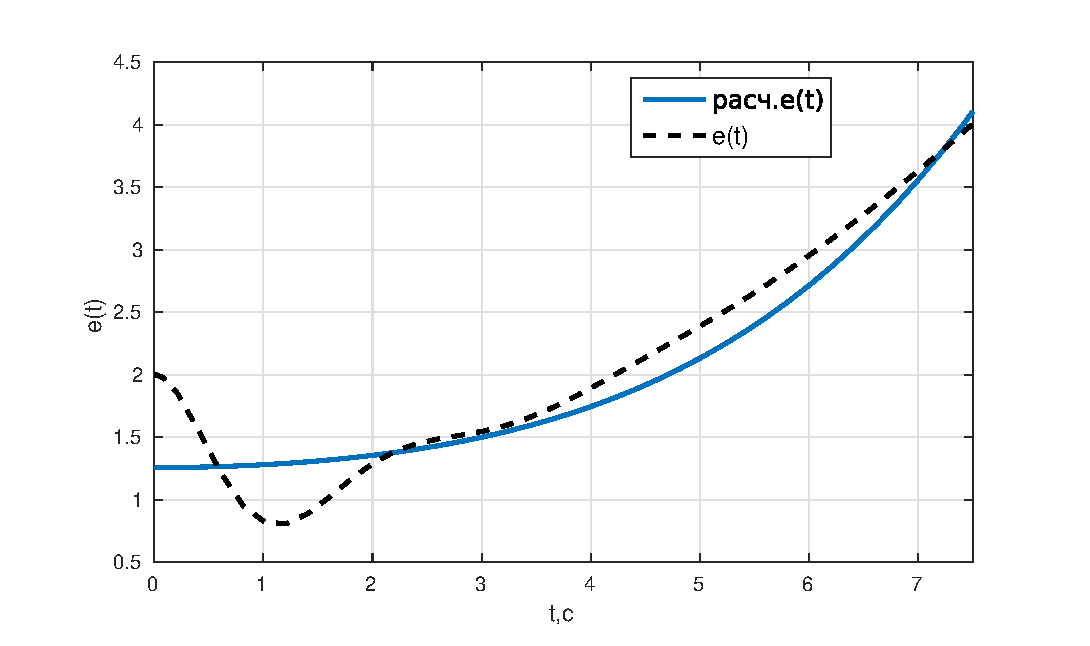
\includegraphics[width=\textwidth]{1/4_2e(t).eps}
\caption{Графики ошибок.}
\end{figure}

\section*{Вывод}
В данной лабораторной работе было проведено исследование системы с астатизмом нулевого и первого порядка; 
исследование влияния внешних возмущений; исследование установившейся ошибки при произвольном входном воздействии.
При исследовании системы с нулевым порядком астатизма в стационарном режиме работы значения установшейся ошибки были больше нуля.
А при исследовании системы с первым порядком астатизма в стационарном режиме работы значения установшейся ошибки стремились к нулю.
Полученные значения установившейся ошибки были проверены аналитически. 
При исследовании установившейся ошибки при произвольном входном воздействии - значение установившейся ошибки стремилось к бесконечности.


\end{document}
